\chapter{Several releases to the same user}\label{ch:programmes}

At the Lisbon workshop where this work was first presented, a participant asked
what happens to the risk when an institution gives several data sets to the same
researcher. The question is the right one to ask, because single releases are not
how institutions publish. A central bank releases a quarterly series, a research
file and a public extract, all drawn from one register, and a researcher with
access to one of them often has access to the others. This chapter shows that the
risk of the combination cannot be read off the risks of the parts, proves that no
rule based only on the parts can bound it, measures the gap on simulated and public
data, and sets out what an institution should assess instead.

\section{Two different questions about a programme}

Let an institution publish releases $Y_1,\dots,Y_m$. For each release let $C_i$ be
the event that the release, used on its own, allows a correct identification under
its declared attack, and let $R_i = \Prob(C_i)$ be its marginal risk. A natural
first question is the probability that at least one release, used alone, exposes
the target, which is the probability of the union
$C_\cup = C_1 \cup \dots \cup C_m$. The marginal risks say something about this
event, though less than one might hope.

\begin{proposition}[Sharp bounds from marginal risks]\label{prop:boole}
Without assumptions on how the events $C_i$ depend on one another,
\begin{equation}\label{eq:boole}
\max_i R_i \ \le\ \Prob(C_\cup)\ \le\ \min\Big(1,\ \sum_{i=1}^m R_i\Big),
\end{equation}
and both bounds are attained by suitable joint distributions, so the marginal risks
alone cannot identify a narrower interval.
\end{proposition}

The interval is wide. If the releases were independent, the union would have
probability $1 - \prod_i (1 - R_i)$, but releases cut from one register are
ordinarily dependent, since they describe the same people, and that expression
needs evidence before it can be used. In the simulation reported below the
independence value is 0.231 inside an interval of $[0.088, 0.253]$. It happens to
sit near the upper bound, and that agreement is a feature of the design and says
nothing about independence.

The second question is the one the participant asked, and it concerns a different
event. An adversary who holds all $m$ releases is not obliged to use them one at a
time. It can apply a joint linkage rule that looks at all the releases together, and
the programme risk is the probability $R_{\mathrm{pool}}$ that this joint rule names
the target. Success of the joint rule is not contained in the union of single-release
successes, so the bounds of Proposition~\ref{prop:boole} do not apply to it.

\section{Pooling intersects candidate sets}

Figure~\ref{fig:pool} shows the mechanism in its smallest form. Each of two
releases groups the target with two other records, so an adversary using either
release alone has a one in three chance. If both releases carry the same pseudonym
for each record, the adversary can keep only the records that appear in both
candidate sets, and here only the target does. Each release is as safe as a key
class of three makes it, and the pair identifies the target with certainty. The sum
of the marginal risks, two thirds, is no bound on the pooled risk.

\begin{figure}[ht]
\centering
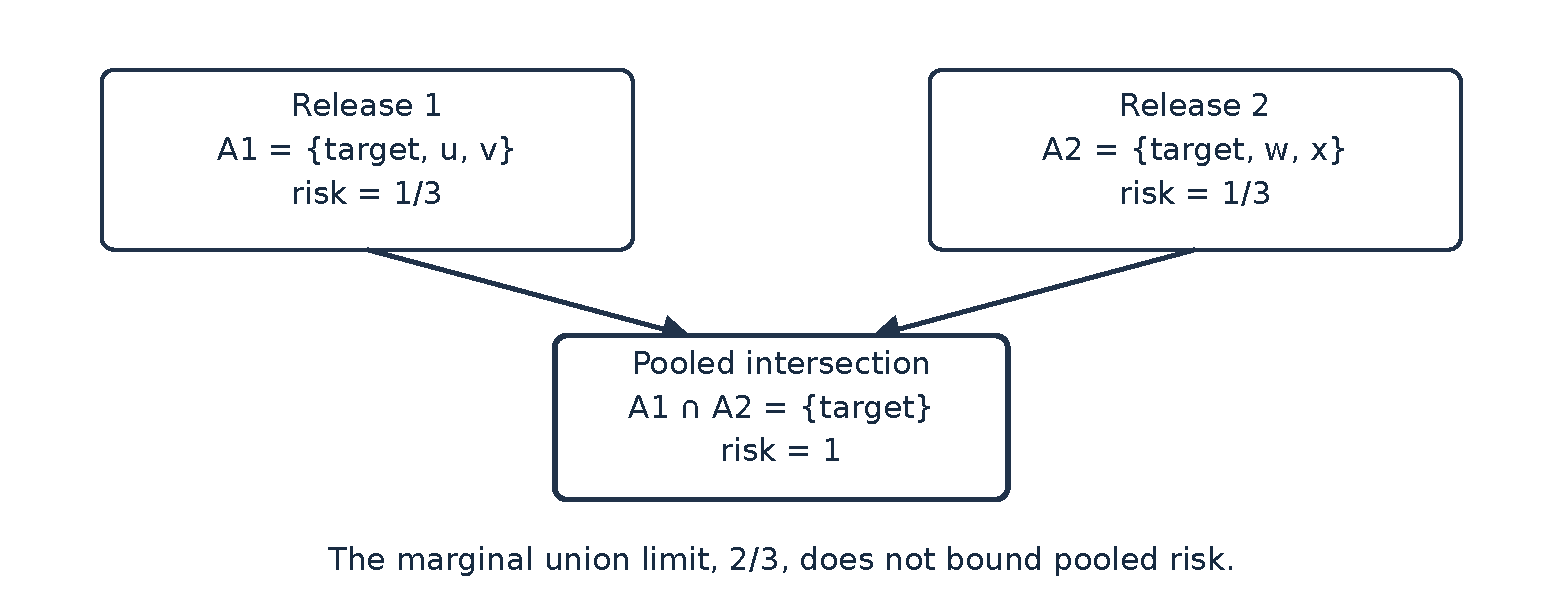
\includegraphics[width=0.78\textwidth]{pooling.pdf}
\caption{Pooling two releases intersects their candidate sets. Each release alone
leaves three candidates for the target; with a pseudonym common to both releases
the adversary keeps only records in both sets, which leaves one.}
\label{fig:pool}
\end{figure}

The small example generalises without limit, which is the central result of the
chapter.

\begin{proposition}[Marginal risks do not bound pooled risk]\label{prop:nopool}
Let $m \ge 2$. Suppose each released record carries a pseudonym that is the same in
every release, and the adversary knows the target's full set of quasi-identifiers,
from which it forms the target's key in every release. For every $\nu > 0$ there
exist a population, a sample and $m$ releases such that $R_i \le \nu$ for every $i$
while $R_{\mathrm{pool}} = 1$. Consequently no upper bound on $R_{\mathrm{pool}}$
can be written as a function of $(R_1,\dots,R_m)$ alone. If each release publishes
the candidate set implied by its key and the adversary chooses uniformly within the
intersection of those sets, then $R_{\mathrm{pool}}$ does not decrease as releases
are added, and $R_{\mathrm{pool}} \ge \max_i R_i$.
\end{proposition}

Neither the phenomenon nor its direction is new. \citet{sweeney2002} observed that
complementary releases, each $k$-anonymous, can be joined to re-identify;
differencing between linked tables is an old problem in disclosure control
\citep[ch.~4]{hundepool2012}; and \citet{ganta2008} showed that independent
releases of overlapping populations, each protected by a syntactic rule, can be
combined into a successful attack. Work on sequential releases of one table
\citep{wang2006,xiao2007} designs protection that survives republication. What the
proposition adds is a statement in the terms an institution uses when it certifies
a release: the quantity a programme is certified against, the per-release risk, is
not the quantity that governs it.

A persistent pseudonym also has a simpler reading. If every release carries the same
pseudonym, the adversary can join the releases into one table keyed on all the
variables any of them publishes. The pooled attack is then an attack on one release
with a finer key, and the proposition says that a finer key can carry far more risk
than any of its parts. That reading points to a remedy as well as a warning, and
Section~\ref{sec:prog-remedies} returns to it.

\section{How large the gap is}

Proposition~\ref{prop:nopool} is an existence result and says nothing about the
size of the gap in a real programme. To measure it, the pipeline draws four
releases from a simulated register of 200,000 units with a 5 per cent sample. Each
release is keyed on ordinary demographic variables, each keeps at least three
records in every key class, and none contains a single unique record. The four share
a record identifier.

Figure~\ref{fig:pool-sim} reports the result. The marginal risks lie between 0.017
and 0.088, so the marginals bound the chance that any one release succeeds between
0.088 and 0.253. An adversary who intersects only the first two releases already
succeeds with probability 0.411, which is 2.8 times the upper bound implied by those
two releases. With all four the pooled risk is 0.458, 1.8 times the bound implied by
all four. A quarter of targets, 26 per cent, are identified uniquely by the
intersection, although none was unique in any single release.

\begin{figure}[ht]
\centering
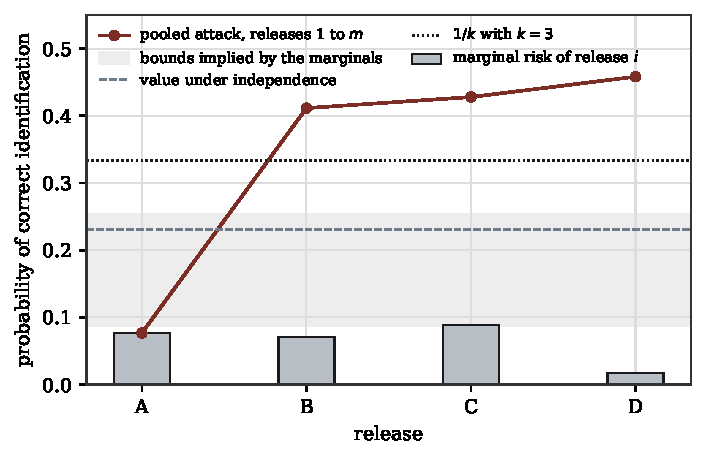
\includegraphics[width=0.8\textwidth]{fig4_composition.pdf}
\caption{Four 3-anonymous releases from one simulated sample: marginal risks, the
interval the marginals imply, and the risk of an adversary that pools releases 1 to
$m$, from 20,000 target replicates. Marginal risks are unconditional, so a target
suppressed from a release contributes zero to it.}
\label{fig:pool-sim}
\end{figure}

The gap is not an artefact of synthetic data. On a public file, an extract of the
US Census 2000 microdata, the same construction gives a pooled risk of 0.709 against
a bound of 0.381 from the marginals. Part~V reports both studies in full.

\section{The credit register}

The running example shows the same effect with an operational lever attached. The
synthetic register releases loans over six monthly vintages, each loan carrying a
persistent pseudonym, its borrower's sector, region and size class, and its
exposure. Judged one release at a time at a tolerance of 0.12, the file passes with
no suppression. The outcome changes once the adversary pools the vintages, but only
under a condition that is worth stating precisely.

\begin{proposition}[Without the history, the other vintages are uninformative]\label{prop:nohistory}
Suppose each loan's published key and exposure are the same in every vintage in
which it appears, that whether a loan is live in a vintage is drawn independently
of its key, its exposure and the adversary's auxiliary information, and that the
adversary knows only that the target is live in the first release. Then, for any
fixed auxiliary information, the adversary's posterior over candidates computed
from all vintages equals its posterior computed from the first vintage alone.
\end{proposition}

The result explains why pooling needs something extra to bite. Repeating the same
published fields adds nothing, and the pattern of months in which each loan is live
carries no information about which loan is the target unless the adversary knows
the target's own pattern. An adversary who does know in which vintages the target's
loan was live, as a counterparty or an informed observer might, can strike out every
candidate whose activity does not match. Against that adversary the decision rule
requires a minimum cell count of 75. An adversary who also holds a reading of the
loan's exposure in each vintage requires 150, and an insider who reads exposure with
small error is not stopped by any floor up to 300.

\section{What to assess instead}\label{sec:prog-remedies}

Three consequences follow for an institution that publishes programmes. First,
marginal risk figures may still be reported, because they describe what an
adversary achieves with one release, but they license no claim about the programme.
Second, a programme must be assessed by simulating the joint attack directly, with
targets and auxiliary information shared across the releases. Separate simulations
of each release cannot recover the dependence between them, because they never form
the intersection. Third, the programme needs a horizon: the number of releases over
which the joint risk is assessed, written into the governance threshold, with a
reassessment due before the next release beyond it. Pooled risk does not decrease as
releases are added, so a programme tolerance without a horizon has no fixed meaning.

The design of the identifier is the second lever. A pseudonym that persists across
releases is what allows the intersection, so rotating it between releases forces any
linkage to run through the published fields instead. The pseudonym itself should be
keyed, for example a keyed hash of the record identifier under a key held apart
from the release team, so that nobody can recompute it from the identifier.
Rotation is a control on linkability and not a guarantee. On the credit register it
does not help while exposure is published exactly, because the published key and
exposure relink every loan from one vintage to the next. With exposure rounded to
one significant figure they relink about one loan in ten. Whether rotation is worth
its cost therefore depends on what else the releases publish, and the joint
simulation is what tells the institution which case it is in.

A formal privacy accountant is the one device that composes across releases without
any assumption about how they depend on one another \citep{dwork2014}. Chapter~10
sets out what that guarantee says and what it leaves unsaid. A programme tolerance
can also be divided among releases as a budget on the union event, but by
Proposition~\ref{prop:nopool} such a budget governs the union only. It allocates
attention across releases and does not replace the joint simulation.

\begin{inpractice}[In practice: giving several files to one user]
List every release from the same register that the user can access, now and within
the assessment horizon, and every identifier or published field that could link
records across them. If records keep a pseudonym across releases, assess the pooled
attack directly by simulation rather than combining per-release figures. Record the
horizon in the decision record and set a reassessment before the first release
beyond it. If the pooled attack fails the tolerance at every acceptable floor,
consider rotating keyed pseudonyms, coarsening the linking fields, or moving the
user to a secure environment, and simulate again for each option.

\smallskip\noindent\textit{In the software.} The bounds and the pooled attack are
in \texttt{privacy\_risk.composition}: \texttt{marginal\_bounds} and
\texttt{independent\_union} for Proposition~\ref{prop:boole}, and
\texttt{pooled\_attack} (or \texttt{pooled\_attack\_from\_sets} for any release
format) for the intersection attack behind Figure~\ref{fig:pool-sim}.
\end{inpractice}

\section{Proofs}

\begin{proof}[Proof of Proposition~\ref{prop:boole}]
Each $C_i$ is contained in $C_\cup$, so $R_i \le \Prob(C_\cup)$ for every $i$, which
gives the lower bound. Subadditivity of probability gives
$\Prob(C_\cup) \le \sum_i R_i$, and $\Prob(C_\cup) \le 1$ always. For attainment of
the lower bound, let the events be nested, with every $C_i$ contained in the one of
largest probability; then $\Prob(C_\cup) = \max_i R_i$. For the upper bound, if
$\sum_i R_i \le 1$ let the events be pairwise disjoint, so that
$\Prob(C_\cup) = \sum_i R_i$; if $\sum_i R_i > 1$, place the events on a probability
space $[0,1)$ with Lebesgue measure as consecutive arcs of lengths $R_i$ wrapped
around the circle, so that together they cover the whole space and
$\Prob(C_\cup) = 1$.
\end{proof}

\begin{proof}[Proof of Proposition~\ref{prop:nopool}]
Fix $\nu > 0$ and choose an integer $k \ge 1/\nu$ with $k \ge 2$. Let the population
and the sample both consist of $k^m$ units, each labelled by a distinct vector
$(v_1,\dots,v_m) \in \{1,\dots,k\}^m$, and let these labels be the units'
quasi-identifiers. Release $i$ publishes every unit with its persistent pseudonym and
a key made of all coordinates except the $i$th. Units share a key in release $i$
exactly when they agree on every coordinate other than $i$, so every key class in
release $i$ has $k$ members, and under Proposition~\ref{prop:recip} of
Chapter~\ref{ch:scenario} the marginal risk of each release is $R_i = 1/k \le \nu$.

The adversary knows the target's label $(v_1,\dots,v_m)$, so in each release it can
find the target's key class and, through the pseudonyms, the corresponding set of
units. A unit in the class of release 1 agrees with the target on coordinates
$2,\dots,m$; a unit in the class of release 2 agrees with it on coordinate 1 and on
coordinates $3,\dots,m$. A unit in both classes therefore agrees with the target on
every coordinate, and since labels are distinct it is the target. The intersection of
the candidate sets is the target alone, so $R_{\mathrm{pool}} = 1$. Since $\nu$ was
arbitrary, any upper bound on $R_{\mathrm{pool}}$ written through the marginals
alone must equal one at marginals as small as we please, so no bound below one
exists.

For the last claim, let $A_i$ be the candidate set of release $i$, which contains the
target. The adversary's set after $j$ releases is $A_1 \cap \dots \cap A_j$, which
contains the target and shrinks as $j$ grows, so the uniform success probability
$1/|A_1 \cap \dots \cap A_j|$ does not decrease. Since the intersection of all the
sets is contained in each $A_i$, $1/|\bigcap_i A_i| \ge 1/|A_i| = R_i$ for every $i$,
and taking expectations over targets gives $R_{\mathrm{pool}} \ge \max_i R_i$.
\end{proof}

\begin{proof}[Proof of Proposition~\ref{prop:nohistory}]
Let $\mathcal{C}$ be the set of candidates the adversary forms from the first
vintage. For a candidate $j$, write $w_j$ for its published key and exposure and
$a_j$ for its pattern of activity across vintages. Under the hypothesis that $j$ is
the target, the joint probability of everything the adversary observes factorises
into a term for its auxiliary information given $w_j$, which is the term the first
vintage alone supplies, and a term for the activity patterns of all loans. The later
vintages contribute only copies of the $w_\ell$, which are already known from the
first, and the patterns $a_\ell$. Since activity is drawn independently of keys,
exposures and auxiliary information, and the adversary knows nothing of the target's
pattern beyond its presence in the first vintage, which every candidate shares, the
activity term is the same for every hypothesis $j \in \mathcal{C}$. It cancels from
the posterior, which therefore equals the posterior computed from the first vintage
alone.
\end{proof}
